\documentclass[a4paper,usenames,dvipsnames, border=0pt]{standalone}

\usepackage{times}      % Loads the Times-Roman Fonts
\usepackage{mathptmx}   % Loads the Times-Roman Math Fonts
\usepackage{subcaption}
\usepackage[labelfont={bf,sf},%
labelsep=period,%
justification=centering,
labelformat=parens,labelsep=quad,skip=3pt,font=scriptsize]{caption}
\usepackage{graphicx}
\usepackage{tikz}
\usetikzlibrary{automata,positioning,arrows,shapes,fit,arrows.meta}
\tikzset{>=latex}
\usepackage{xcolor}
\definecolor{dodgerblue}{RGB}{30,144,255}
\definecolor{silver}{RGB}{192,192,192}

\begin{document}
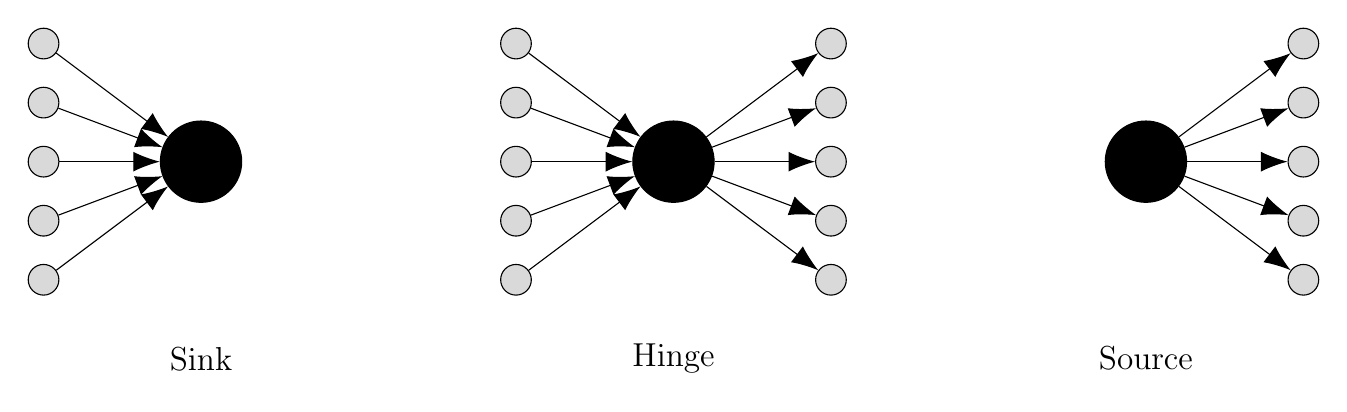
\begin{tikzpicture}[shorten >=0pt,node distance=0.75cm and 3cm,on grid,auto] 
	\large
\node[state] (hinge) [align=center,fill=black] {};
\node[state] (sink) [align=center,fill=black, left=6cm of hinge] {};
\node[state] (source) [align=center,fill=black, right=6cm of hinge] {};
\node[circle,draw=black] (v1) [fill=gray!30,left=2cm of sink,] {};
\node[circle,draw=black] (v2) [fill=gray!30,above= of v1,] {};
\node[circle,draw=black] (v3) [fill=gray!30,above= of v2,] {};
\node[circle,draw=black] (v4) [fill=gray!30,below= of v1,] {};
\node[circle,draw=black] (v5) [fill=gray!30,below= of v4,] {};
\node[circle,draw=black] (w1) [fill=gray!30,left=2cm of hinge,] {};
\node[circle,draw=black] (w2) [fill=gray!30,above= of w1,] {};
\node[circle,draw=black] (w3) [fill=gray!30,above= of w2,] {};
\node[circle,draw=black] (w4) [fill=gray!30,below= of w1,] {};
\node[circle,draw=black] (w5) [fill=gray!30,below= of w4,] {};
\node[circle,draw=black] (x1) [fill=gray!30,right=2cm of hinge,] {};
\node[circle,draw=black] (x2) [fill=gray!30,above= of x1,] {};
\node[circle,draw=black] (x3) [fill=gray!30,above= of x2,] {};
\node[circle,draw=black] (x4) [fill=gray!30,below= of x1,] {};
\node[circle,draw=black] (x5) [fill=gray!30,below= of x4,] {};
\node[circle,draw=black] (y1) [fill=gray!30,right=2cm of source,] {};
\node[circle,draw=black] (y2) [fill=gray!30,above= of y1,] {};
\node[circle,draw=black] (y3) [fill=gray!30,above= of y2,] {};
\node[circle,draw=black] (y4) [fill=gray!30,below= of y1,] {};
\node[circle,draw=black] (y5) [fill=gray!30,below= of y4,] {};
\node (sinklabel) [below=2.5cm of sink] {Sink};
\node (hingelabel) [below=2.5cm of hinge] {Hinge};
\node (sourcelabel) [below=2.5cm of source] {Source};
\path[-{Latex[scale=2.0]}]
(v1) edge [align=center] (sink)
(v2) edge [align=center] (sink)
(v3) edge [align=center] (sink)
(v4) edge [align=center] (sink)
(v5) edge [align=center] (sink)
(w1) edge [align=center] (hinge)
(w2) edge [align=center] (hinge)
(w3) edge [align=center] (hinge)
(w4) edge [align=center] (hinge)
(w5) edge [align=center] (hinge)
(hinge) edge [align=center] (x1)
(hinge) edge [align=center] (x2)
(hinge) edge [align=center] (x3)
(hinge) edge [align=center] (x4)
(hinge) edge [align=center] (x5)
(source) edge [align=center] (y1)
(source) edge [align=center] (y2)
(source) edge [align=center] (y3)
(source) edge [align=center] (y4)
(source) edge [align=center] (y5)
;
\end{tikzpicture}
\end{document}